\section{Kernel Methods}

\subsection{Introduction}

A \textbf{classifier} is a mapping \(\hat{c} : \mathcal{X} \to \mathcal{C}\), where \(\mathcal{C} = \{C_1, C_2, \dots, C_k\}\) is a finite and usually small set of \textbf{class labels}. We use the `hat' to indicate that \(\hat{c}(x)\) is an estimate of the true but unknown function \(c(x)\). \\

A \textbf{scoring classifier} is a mapping \(\hat{\mathbf{s}} : \mathbf{\mathcal{X}} \to \mathbb{R}^k\), i.e., a mapping from the instance space to a \(k\)-vector of real numbers. The boldface notation indicates that a vector \(\hat{\mathbf{s}}(x) = (\hat{s}_1(x), \dots, \hat{s}_k(x))\) rather than a single number; \(\hat{s}_i(x)\) is the score assigned to class \(C_i\) for instance \(x\). \\

If we take the true class \(c(x)\) as \(+1\) for positive examples and \(-1\) for negative examples, then the quantity \(z(x) = c(x)\hat{s}(x)\) is positive for  correct predictions and negative for incorrect predictions: this quantity is called the \textbf{margin} assigned by the scoring classifier to the example. \\

We would like to reward large positive margins, and penalise large negative values. This is achieved by a means of a so-called \textbf{loss function} \(L: \mathbb{R} \to [0, \infty)\) which maps each example's margin \(z(x)\) to an associated loss \(L(z(x))\).

\subsection{Dual Perceptron}

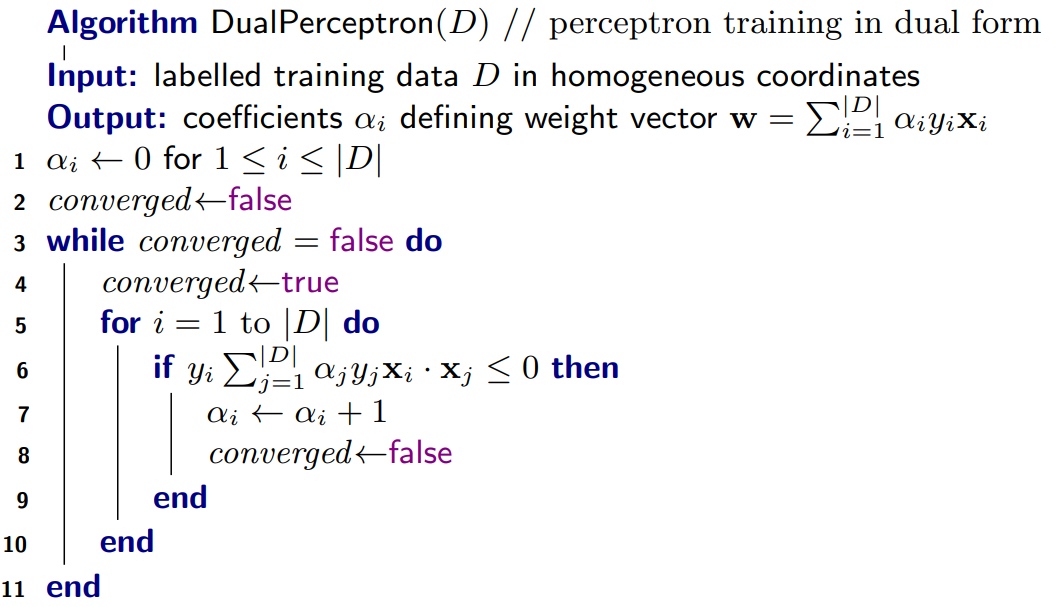
\includegraphics[scale=0.6]{./assets/dual_perceptron.png}

\subsection{Support Vector Machines}

A bunch of math, look at the lecture slides. TLDR is finds optimal hyperplanes which best separates the data into different classes by maximising the margin between them.

\subsection{The Kernel Trick}

Let \(\vecx_1 = (x_1, y_1)\) and \(\vecx_2 = (x_2, y_2)\) be two data points, and consider the mapping \((x, y) \mapsto (x^2, y^2, \sqrt{2}xy)\) to a three-dimensional feature space. The points in feature space corresponding to \(\vecx_1\) and \(\vecx_2\) are \(\vecx_1' = (x_1^2, y_1^2, \sqrt{2}x_1y_1)\) and \(\vecx_2' = (x_2^2, y_2^2, \sqrt{2}x_2y_2)\). The dot product of these two feature vectors is

\[\vecx_1' \cdot \vecx_2' = x_1^2x_2^2 + y_1^2y_2^2 + 2x_1y_1x_2y_2 = (x_1x_2 + y_1y_2)^2 = (\vecx_! \cdot \vecx_2)^2.\]

That is, by squaring the dot product in the original space we obtain the dot product in the new space without actually constructing the feature vectors! A function that calculates the dot product in feature space directly from the vectors in the original space is called a \textbf{kernel} - here the kernel is \(\mathbf{\kappa}(\vecx_1, \vecx_2) = (\vecx_1 \cdot \vecx_2)^2\). \\

The mapping function \(\phi(\vecx)\) maps the data to a different space. The idea is that learning, say, a linear separator, can be easier in this space. \\

The kernel function \(\mathbf{\kappa}(\vecx_i, \vecx_j) = \phi(\vecx_i) \cdot \phi(\vecx_j)\) replaces \(\vecx_i \cdot \vecx_j\).

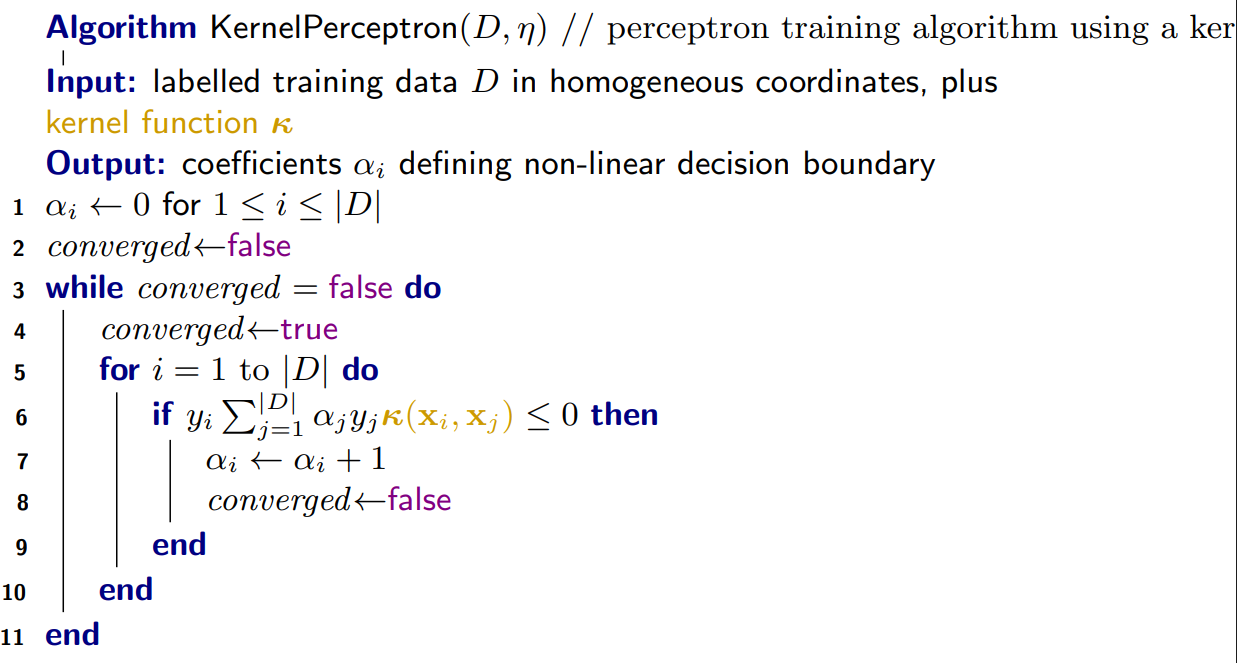
\includegraphics[scale=0.6]{./assets/kernel_perceptron.png}
